% Created 2018-09-26 Wed 11:38
% Intended LaTeX compiler: pdflatex
\documentclass[presentation]{beamer}
\usepackage[utf8]{inputenc}
\usepackage[T1]{fontenc}
\usepackage{graphicx}
\usepackage{grffile}
\usepackage{longtable}
\usepackage{wrapfig}
\usepackage{rotating}
\usepackage[normalem]{ulem}
\usepackage{amsmath}
\usepackage{textcomp}
\usepackage{amssymb}
\usepackage{capt-of}
\usepackage{natbib}
\usepackage[linktocpage,pdfstartview=FitH,colorlinks,
linkcolor=blue,anchorcolor=blue,
citecolor=blue,filecolor=blue,menucolor=blue,urlcolor=blue]{hyperref}
\setbeamertemplate{frame footer}{\insertshortauthor}
\setbeamerfont{page number in head/foot}{size=\tiny}
\setbeamercolor{footline}{fg=gray}
\author{Florian Hollenbach}
\usepackage[english]{isodate}
\usepackage{amsmath,amsthm,amssymb,amsfonts}
\usetheme{metropolis}
\usecolortheme{}
\usefonttheme{}
\useinnertheme{}
\useoutertheme{}
\author{Florian Hollenbach}
\date{\today}
\title{Political Science 209 - Fall 2018}
\subtitle{Measurement}

\hypersetup{
 pdfauthor={Florian Hollenbach},
 pdftitle={Political Science 209 - Fall 2018},
 pdfkeywords={},
 pdfsubject={},
 pdfcreator={Emacs 25.3.1 (Org mode 9.1.9)}, 
 pdflang={English}}
\begin{document}

\maketitle

\begin{frame}[label={sec:org8e4117d}]{Survey Sampling}
\begin{itemize}
\item A sample is a small share of the population in that we are interested in
\end{itemize}

\pause

\begin{itemize}
\item How do we draw samples in such a way that polls accurately reflect what is going to happen?

\item How to construct samples that will represent the population?
\end{itemize}
\end{frame}

\begin{frame}[label={sec:org8d12559}]{Survey Sampling}
\begin{itemize}
\item Example: We want to know the voting intentions of Texans (or Americans)
\item We can hardly ask all eligible voters about their intention
\end{itemize}

\pause
\begin{itemize}
\item We take a \emph{sample}
\end{itemize}
\end{frame}

\begin{frame}[label={sec:org6a5ef9d}]{Survey Sampling}
\begin{itemize}
\item The size of the sample is less important than its composition
\end{itemize}

\begin{center}
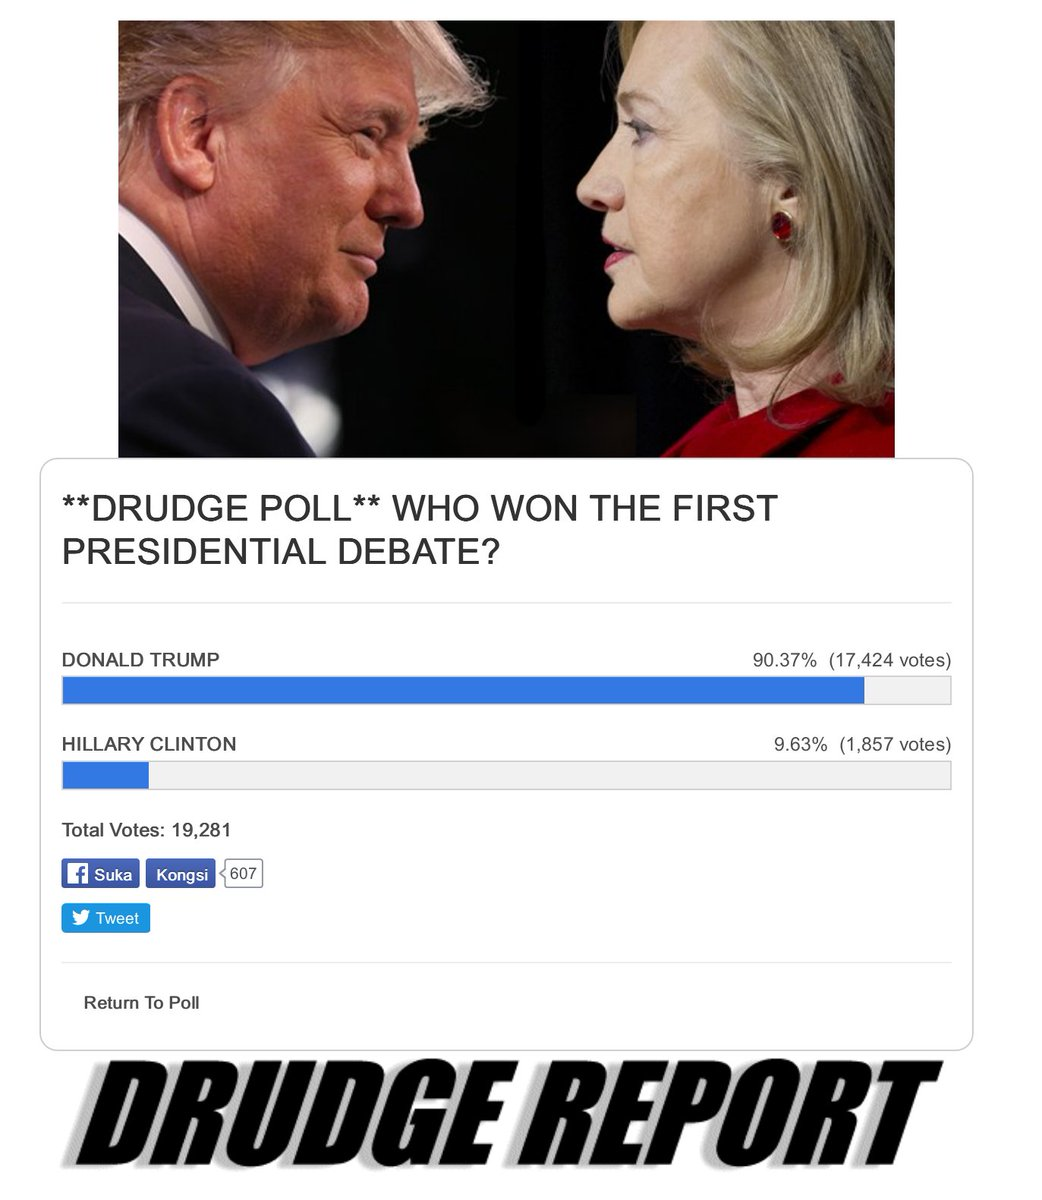
\includegraphics[width=8cm]{/Users/florianhollenbach/Documents/GitHub/Polisci209_2018/slides/week5/drudge.jpeg}
\end{center}

\begin{itemize}
\item Never trust an internet poll
\end{itemize}
\end{frame}

\begin{frame}[label={sec:orgd04d9bd}]{Literary Digest Sample}
\begin{itemize}
\item Mail questionnaire to 10 million people

\item Addresses came from phone books and club memberships

\item Problems?
\end{itemize}

\pause

\begin{itemize}
\item Biased \emph{sample}
\end{itemize}
\end{frame}


\begin{frame}[label={sec:orgf06f198}]{Quota Samping}
\begin{itemize}
\item Sample certain groups until quota is filled

\item Does not mean unobservables are representative
\end{itemize}
\end{frame}

\begin{frame}[label={sec:org24238ca}]{Simple Random Sampling}
\begin{itemize}
\item Think of all voters sitting in a box, survey firm randomly draws voters

\item Random draws without replacement give us an unbiased estimate of the population

\item Everybody has the same chance of being in the sample
\end{itemize}
\end{frame}


\begin{frame}[label={sec:org7f2debc}]{Simple Random Sampling}
\begin{itemize}
\item Pre-determined number of units are randomly selected from population

\item Sample will be representative of population on observed and unobserved characteristics
\end{itemize}
\end{frame}



\begin{frame}[label={sec:org9d7e69e}]{Simple Random Sampling}
\begin{itemize}
\item Not every single sample will be exactly representative

\item If we were to take a lot of random samples (say 1000 samples of 1000 respondents), on average the samples would be representative
\end{itemize}
\end{frame}

\begin{frame}[label={sec:orgabf1288}]{Simple Random Sampling}
\begin{itemize}
\item Each single sample can be off and different

\item Polls are associated with uncertainty
\end{itemize}

\begin{center}
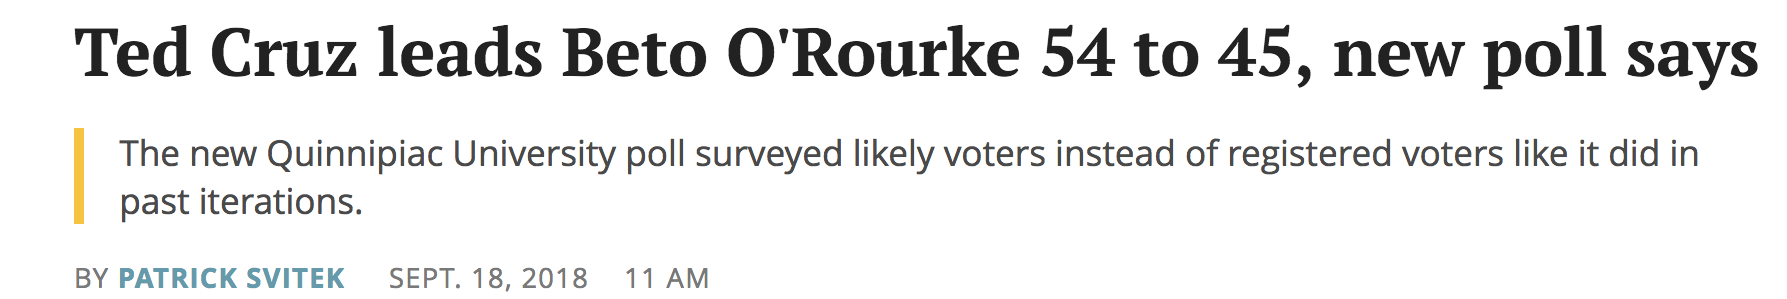
\includegraphics[width=8cm]{/Users/florianhollenbach/Documents/GitHub/Polisci209_2018/slides/week5/cruz.png}
\end{center}

\pause


\begin{center}
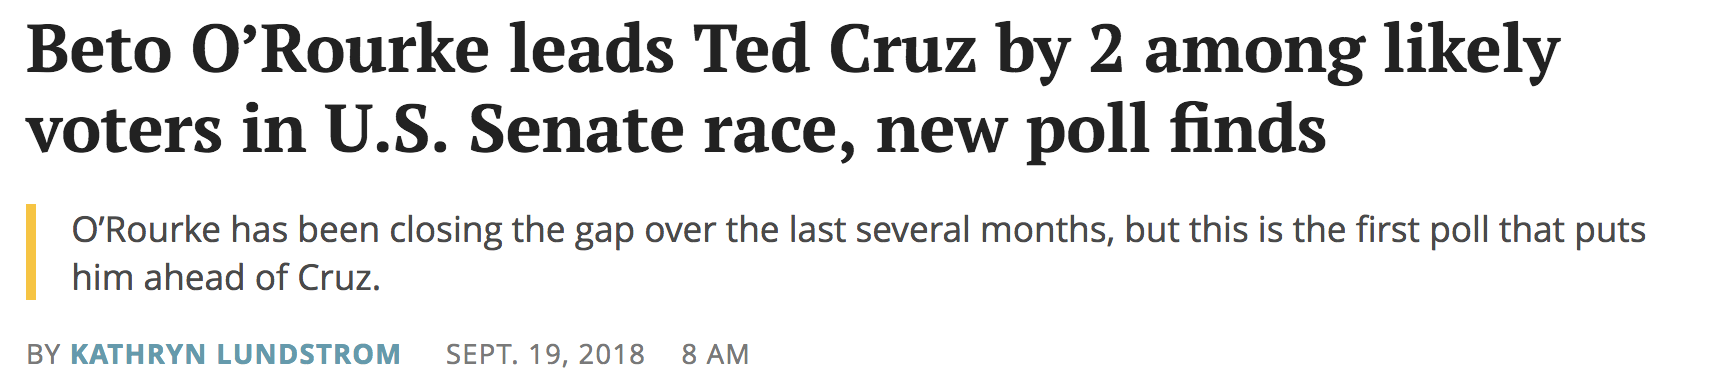
\includegraphics[width=8cm]{/Users/florianhollenbach/Documents/GitHub/Polisci209_2018/slides/week5/orourke.png}
\end{center}
\end{frame}


\begin{frame}[label={sec:orge7d80b9}]{Random Sampling is hard}
\begin{itemize}
\item How to create sampling frame?

\item Random digit dialing? Walking to random houses?

\item Multi-stage cluster sampling
\end{itemize}
\end{frame}

\begin{frame}[label={sec:org4bf4069}]{Non-reponse bias}
\begin{itemize}
\item Unit non-response bias:
\end{itemize}

\begin{center}
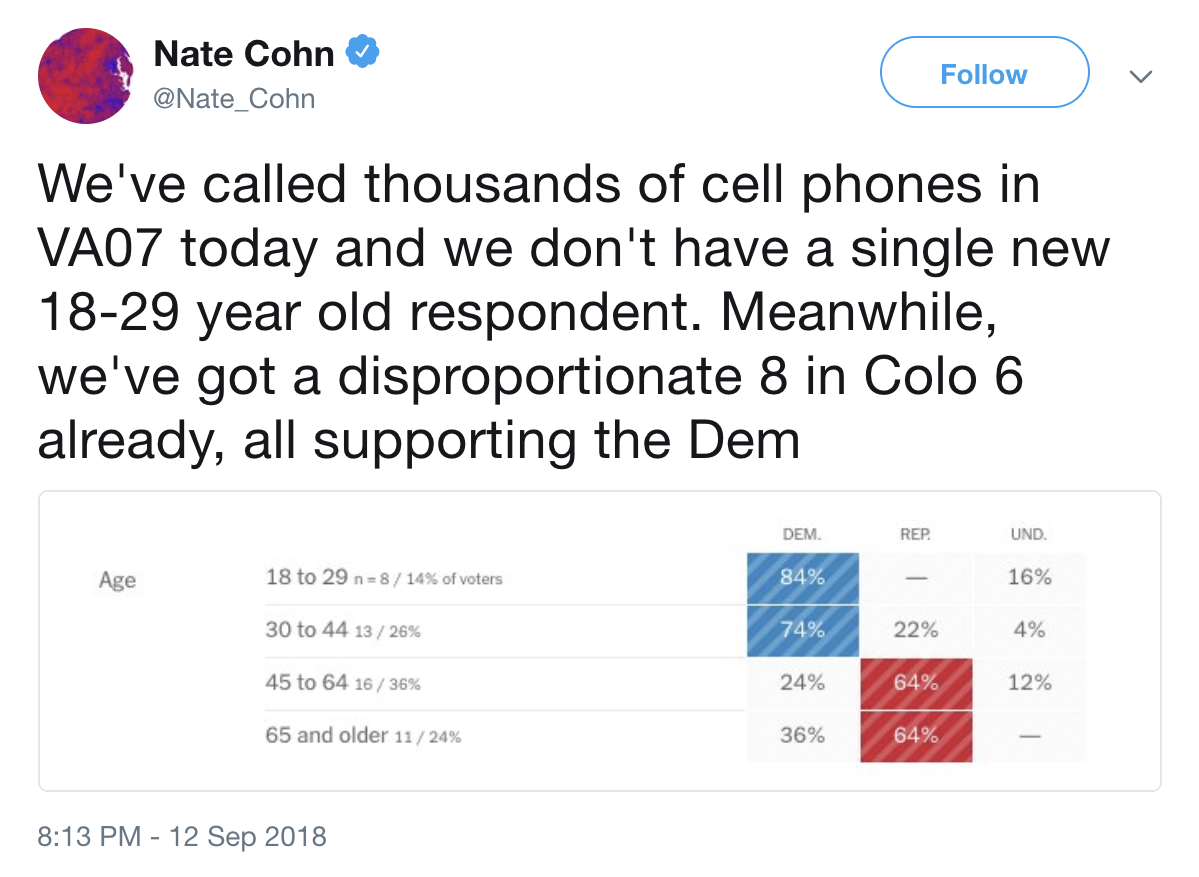
\includegraphics[width=8cm]{/Users/florianhollenbach/Documents/GitHub/Polisci209_2018/slides/week5/cohn.png}
\end{center}
\end{frame}




\begin{frame}[label={sec:org37decaf}]{Non-reponse bias}
\begin{itemize}
\item Item non-response bias:
\emph{What was the last crime you committed?}
\item Sensitive questions: non-response, social desirability bias
\emph{Turnout}, \emph{racial prejudice}, \emph{corruption}
\end{itemize}
\end{frame}


\begin{frame}[label={sec:orgec29665}]{Why could this be a problem in the Afghanistan example?}
\begin{center}
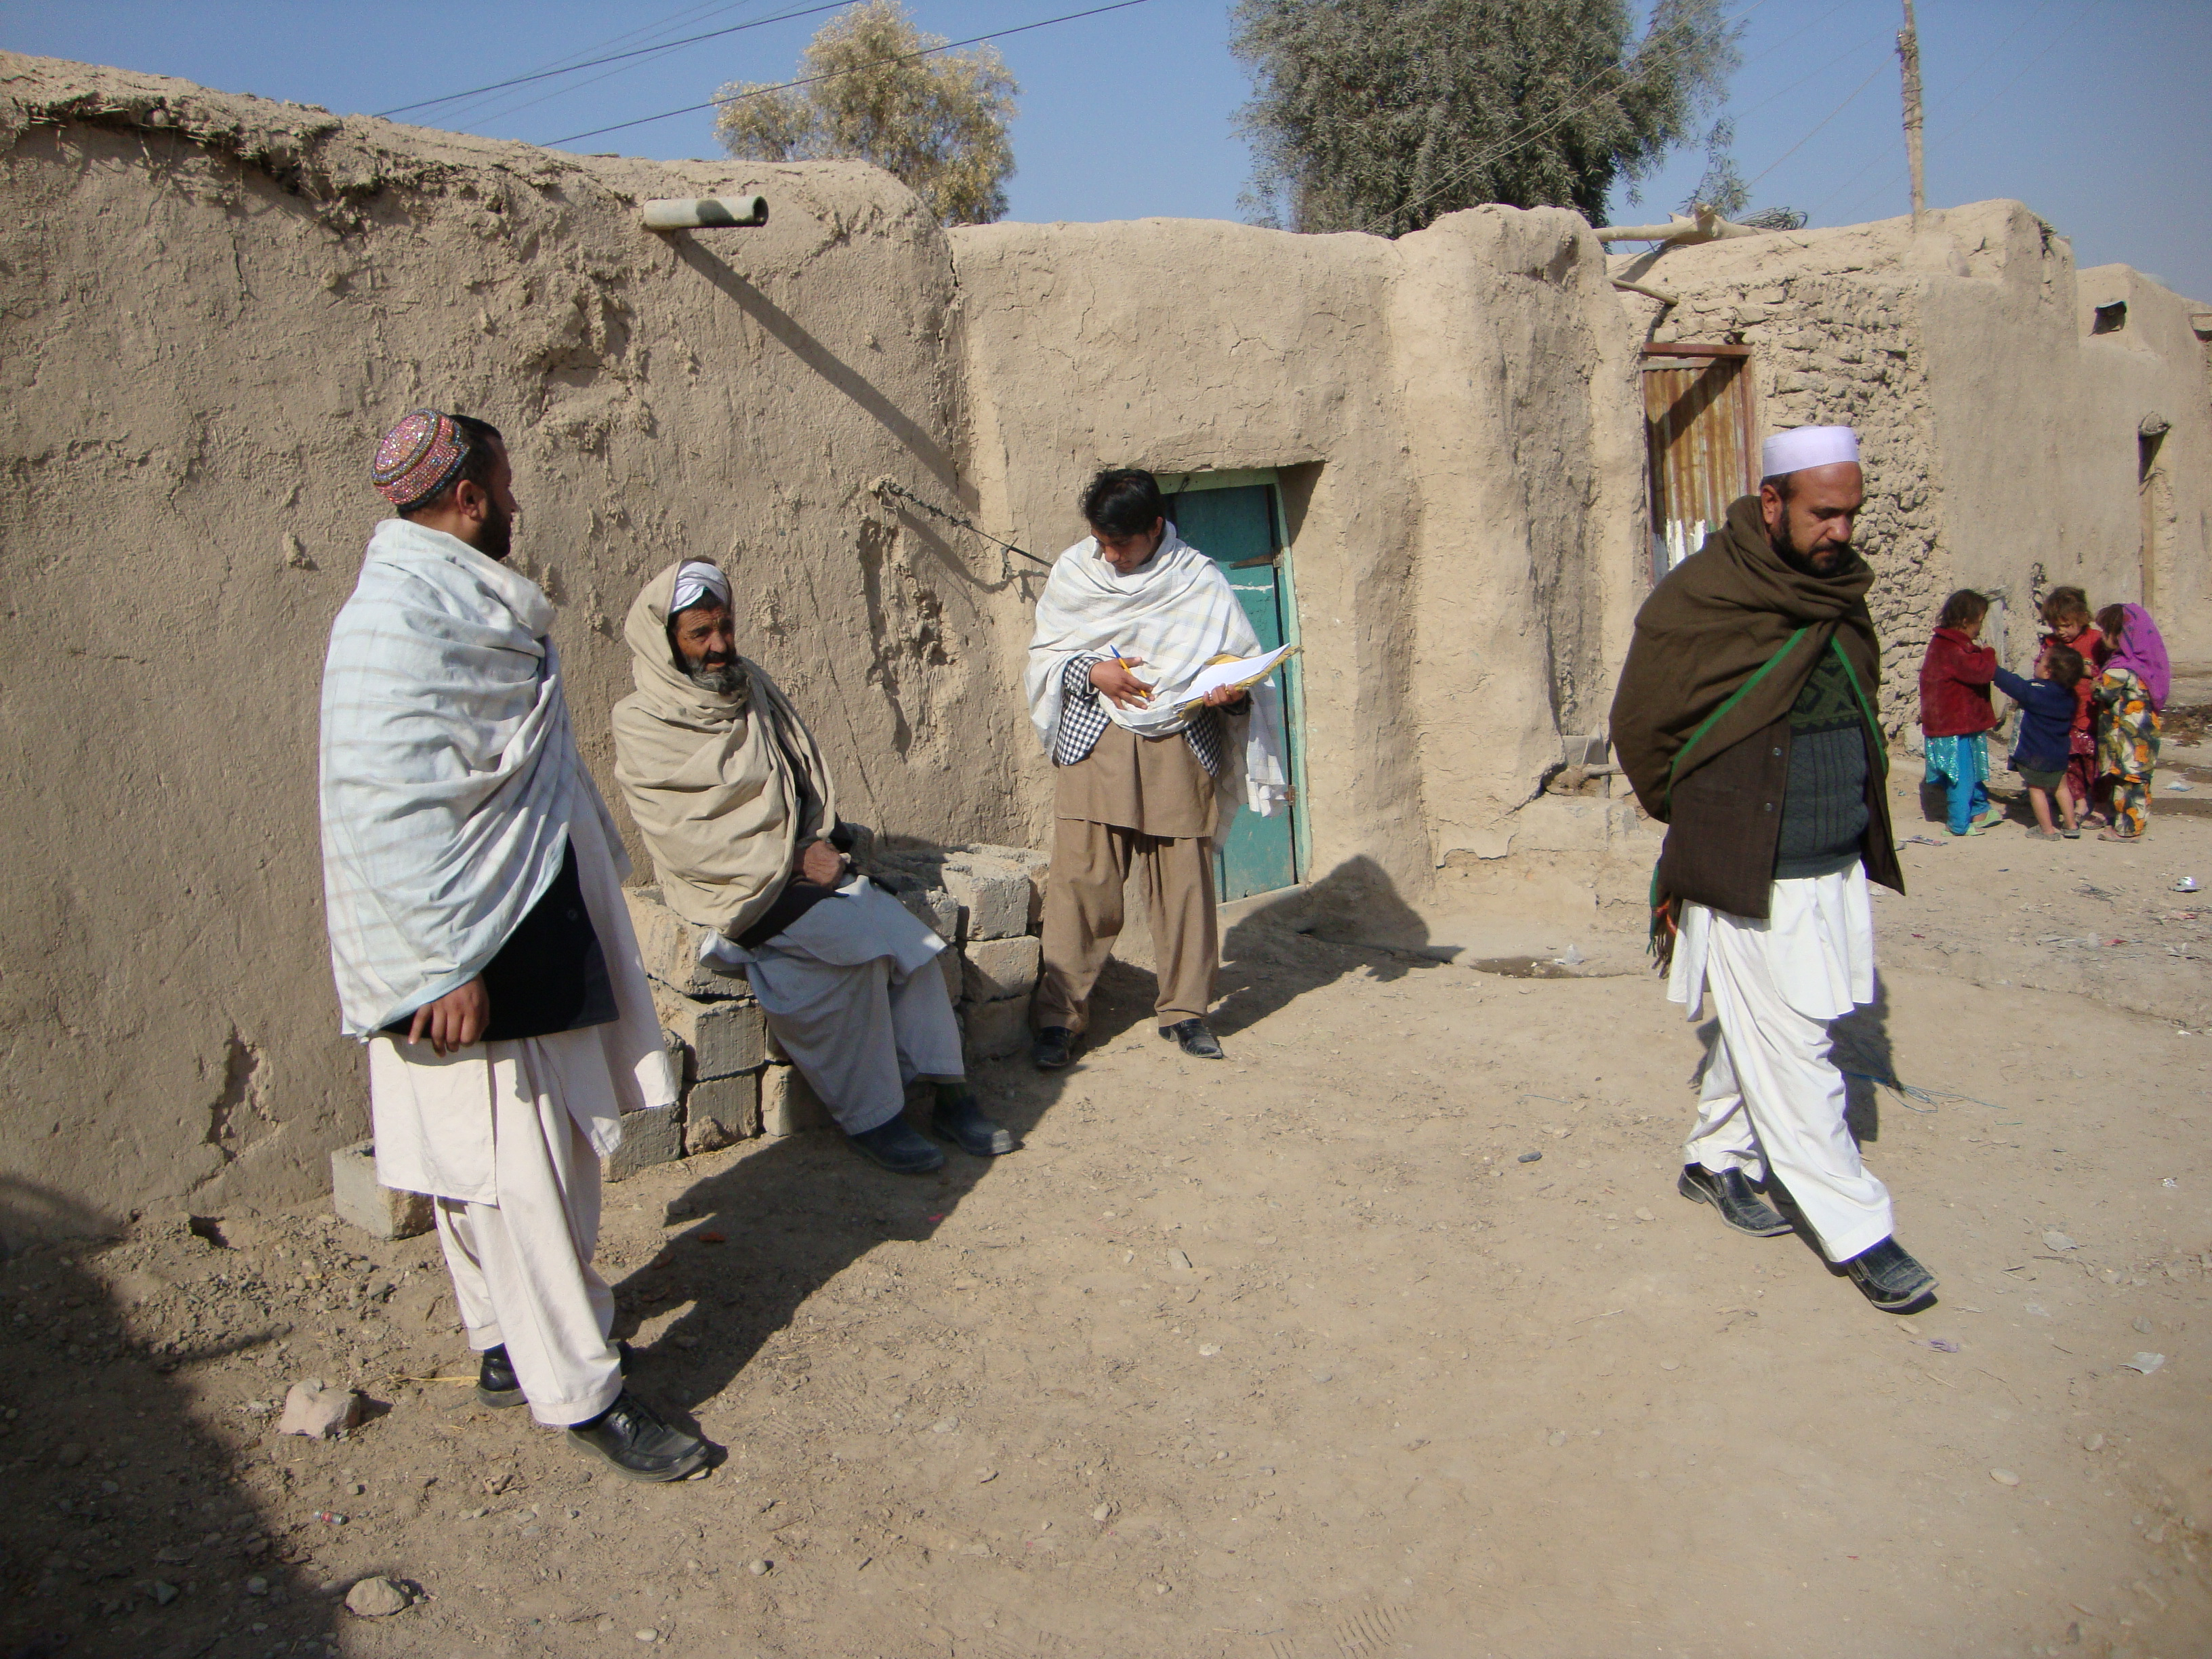
\includegraphics[width=8cm]{/Users/florianhollenbach/Documents/GitHub/Polisci209_2018/slides/week5/afghan-survey.jpg}
\end{center}
\end{frame}

\begin{frame}[label={sec:orgdab6389}]{Examples of Problems of Running Surveys in Afghanistan}
\begin{itemize}
\item unit non-response bias:
\end{itemize}
\pause
\emph{some citizens might not want to anser the door}

\pause
\begin{itemize}
\item item non-response bias:
\end{itemize}
\pause
\emph{Taliban supporters may be less likely to answer questions about Taliban}

\pause
\begin{itemize}
\item social desirability bias:
\end{itemize}
\pause
\emph{Taliban supporters may not want to admit to supporting Taliban}
\end{frame}


\begin{frame}[label={sec:orgdfb9c83}]{Strategies to Ask Sensitive Questions}
\Large{List Experiments}

\begin{itemize}
\item list of groups respondent might support
\item Asked to name number of groups they support
\item Treated subject with controversial group, control group without controversial group
\end{itemize}
\end{frame}


\begin{frame}[shrink=30,label={sec:orgab05091}]{Strategies to Ask Sensitive Questions}
\Large{List Experiments - Control}

I’m going to read you a list with the names of different
groups and individuals on it.  After I read the entire
list, I’d like you to tell me how many of these groups
and individuals you broadly support, meaning that you
generally agree with the goals and policies of the group
or individual.  Please don’t tell me which ones you
generally agree with; only tell me how many groups or
individuals you broadly support.

Groups: Karzai Government; National Solidarity Program; Local
Farmers
\end{frame}

\begin{frame}[shrink=30,label={sec:orgf69a7e7}]{Strategies to Ask Sensitive Questions}
\Large{List Experiments - Treated}

I’m going to read you a list with the names of different
groups and individuals on it.  After I read the entire
list, I’d like you to tell me how many of these groups
and individuals you broadly support, meaning that you
generally agree with the goals and policies of the group
or individual.  Please don’t tell me which ones you
generally agree with; only tell me how many groups or
individuals you broadly support.

Groups: Karzai Government; National Solidarity Program; Local
Farmers; \alert{ISAF (Taliban)}
\end{frame}

\begin{frame}[label={sec:org4497b67}]{Strategies to Ask Sensitive Questions}
\Large{List Experiments}

\begin{itemize}
\item Average difference between Treated and Control group is the estimated percentage of people who support controversial group
\end{itemize}
\end{frame}


\begin{frame}[label={sec:org5c4c4ee}]{Summarizing Bivariate Relationships}
\begin{itemize}
\item Bivariate relationships are associations between \alert{two} variables
\item Example: treatment of Spanish confederates (X or T) and exclusionary attitudes (Y)
\end{itemize}
\end{frame}

\begin{frame}[label={sec:orge311f7a}]{Simple Summaries of Bivariate Relationships}
If X (independent variable) is categorical:
\begin{itemize}
\item Comparison of means
\item boxplots
\end{itemize}
\end{frame}

\begin{frame}[label={sec:orgbe8e651}]{Simple Summaries of Bivariate Relationships}
If both X (independent variable) and Y (dependent variable) are continuous:

\pause
\begin{itemize}
\item Scatterplots
\end{itemize}

\pause
\begin{itemize}
\item Correlation
\end{itemize}
\end{frame}

\begin{frame}[label={sec:orgd492b6c}]{Simple Summaries of Bivariate Relationships: Scatterplot}
\begin{itemize}
\item Direct graphical comparison of two variables

\item Use plot(y,x) in \emph{R}
\end{itemize}
\end{frame}

\begin{frame}[fragile,label={sec:org872ab17}]{Scatterplot}
 \begin{verbatim}
data <- read.csv("bivariate_data.csv")
data <- subset(data, year == 2010)
plot(data$GDP,data$Child.Mortality)
\end{verbatim}
\end{frame}

\begin{frame}[label={sec:org6022ba1}]{Scatterplot}
That looks weird, no? What do we do with skewed variables?
\begin{center}
\includegraphics[width=8cm]{/Users/florianhollenbach/Documents/GitHub/Polisci209_2018/slides/week5/scatter_simple.pdf}
\end{center}
\end{frame}

\begin{frame}[label={sec:org21504de}]{What do we do with skewed variables?}
\pause
\begin{itemize}
\item When variable have a small number of observations with extremely large or small positive values, we often take the natural log
\item The natural logarithm is the logarithm with base e, which is a mathematical constant approximately equal to 2.7182 (inverse of \(e^{y}\))
\end{itemize}
\end{frame}


\begin{frame}[fragile,label={sec:orge862688}]{Scatterplot}
 \begin{verbatim}
plot(log(data$GDP),data$Child.Mortality)
\end{verbatim}
\end{frame}

\begin{frame}[label={sec:orgde1177e}]{Scatterplot}
\begin{center}
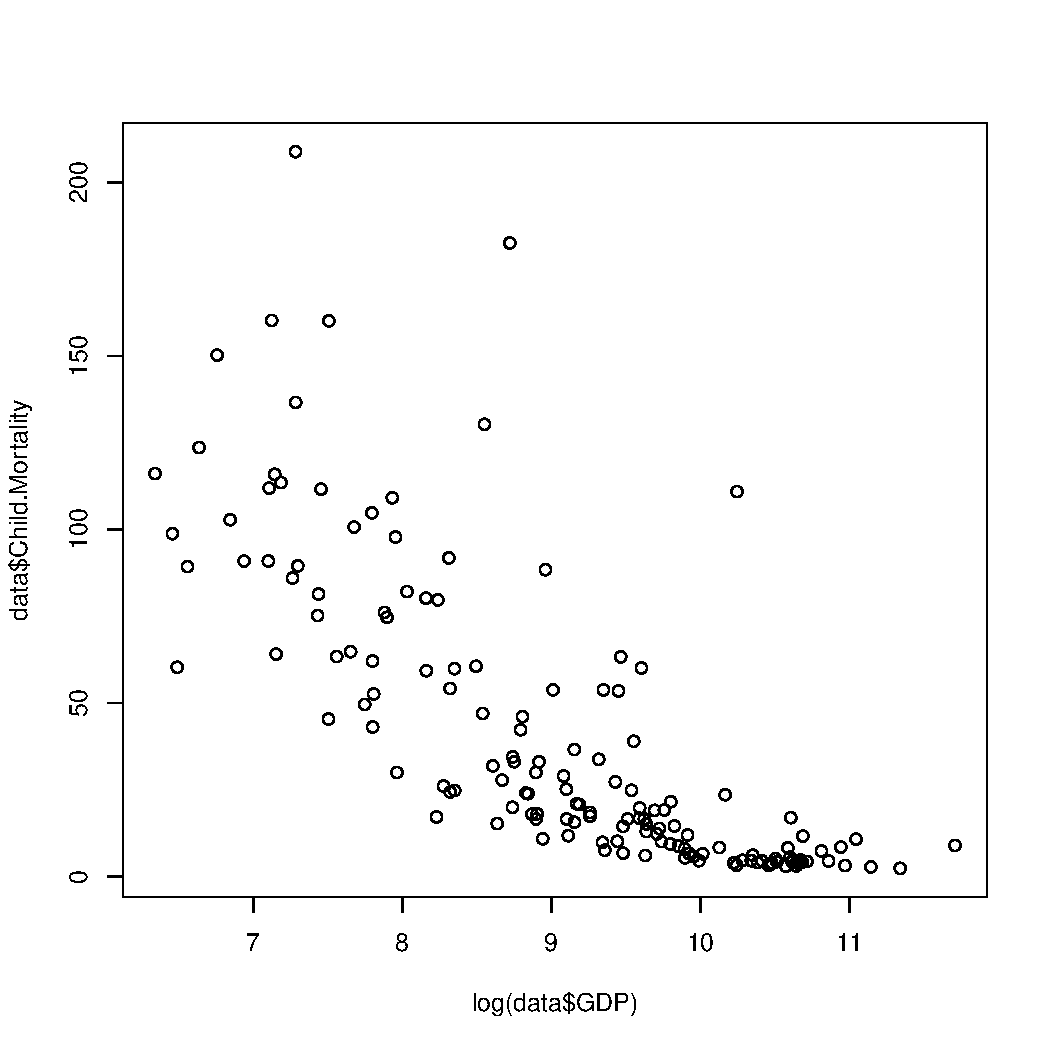
\includegraphics[width=8cm]{/Users/florianhollenbach/Documents/GitHub/Polisci209_2018/slides/week5/scatter_log_simple.pdf}
\end{center}

\Large{Better!}
Let's add labels and nicer points
\end{frame}


\begin{frame}[fragile,shrink=35,label={sec:orgac518d1}]{Scatterplot}
 \begin{verbatim}
pdf("~/Documents/GitHub/Polisci209_2018/slides/week5/scatter.pdf")
plot(log(data$GDP),data$Child.Mortality, pch = 16, col = "black",
xlab = "logged GDP in PPP", ylab = "Child Mortality", main = "Income and Child Mortality")
dev.off()
\end{verbatim}
\end{frame}

\begin{frame}[label={sec:orge1194e0}]{Scatterplot}
\begin{center}
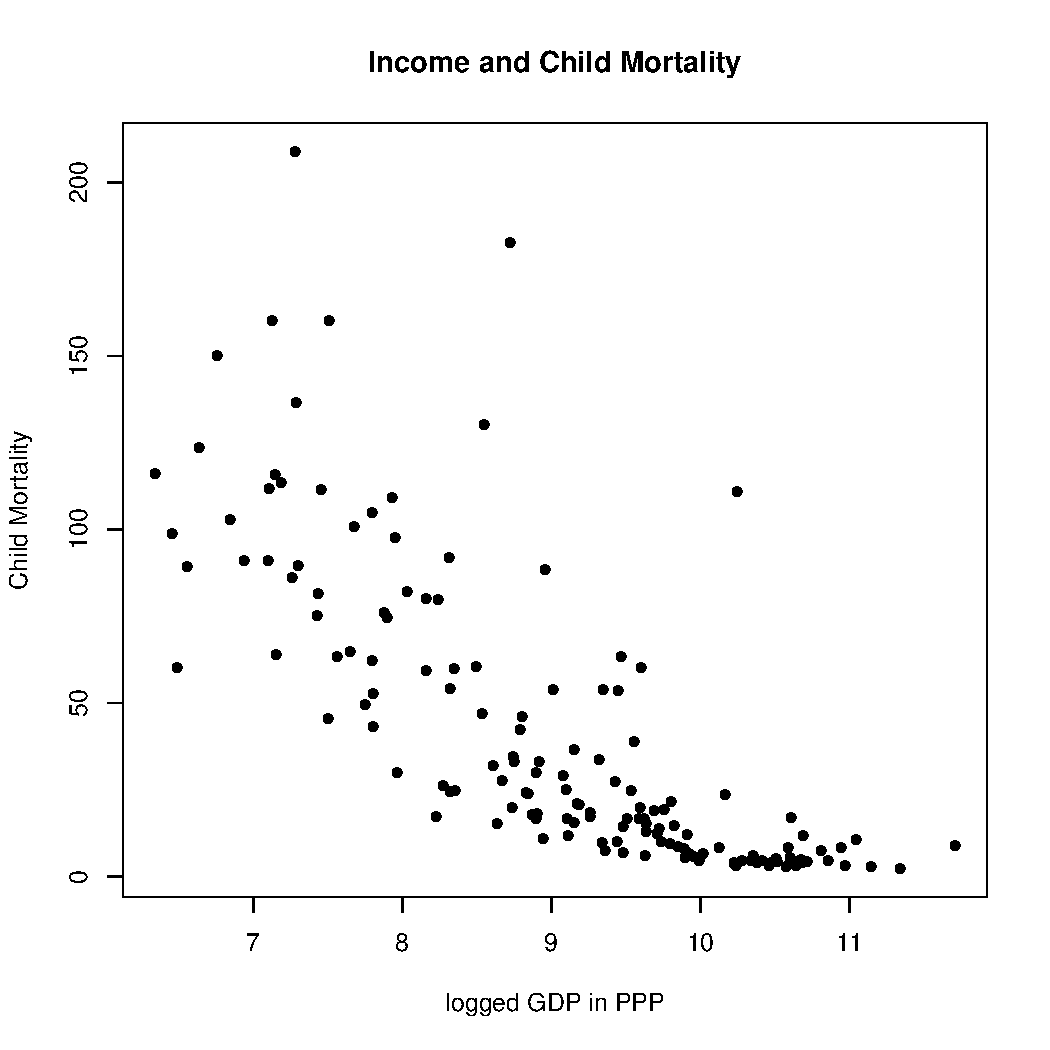
\includegraphics[width=8cm]{/Users/florianhollenbach/Documents/GitHub/Polisci209_2018/slides/week5/scatter.pdf}
\end{center}
\end{frame}

\begin{frame}[fragile,shrink=55,label={sec:org5d021f9}]{Scatterplot -- more fun}
 \begin{verbatim}
## add special points for USA and Germany
pdf("~/Documents/GitHub/Polisci209_2018/slides/week5/scatter_points.pdf")
plot(log(data$GDP),data$Child.Mortality, pch = 16, col = "black",
xlab = "logged GDP in PPP", ylab = "Child Mortality", main = "Income and Child Mortality")
points(log(data$GDP[data$Country.code == "USA"]), data$Child.Mortality[data$Country.code == "USA"], pch = 17, col = "red") ##USA
text(11, 16, "USA", col = "red")
points(log(data$GDP[data$Country.code == "DEU"]), data$Child.Mortality[data$Country.code == "DEU"], pch = 15, col = "gold") ##USA
text(10.2, 0, "GER", col = "gold")
dev.off()
\end{verbatim}
\end{frame}


\begin{frame}[label={sec:orgb6949bb}]{Scatterplot}
\begin{center}
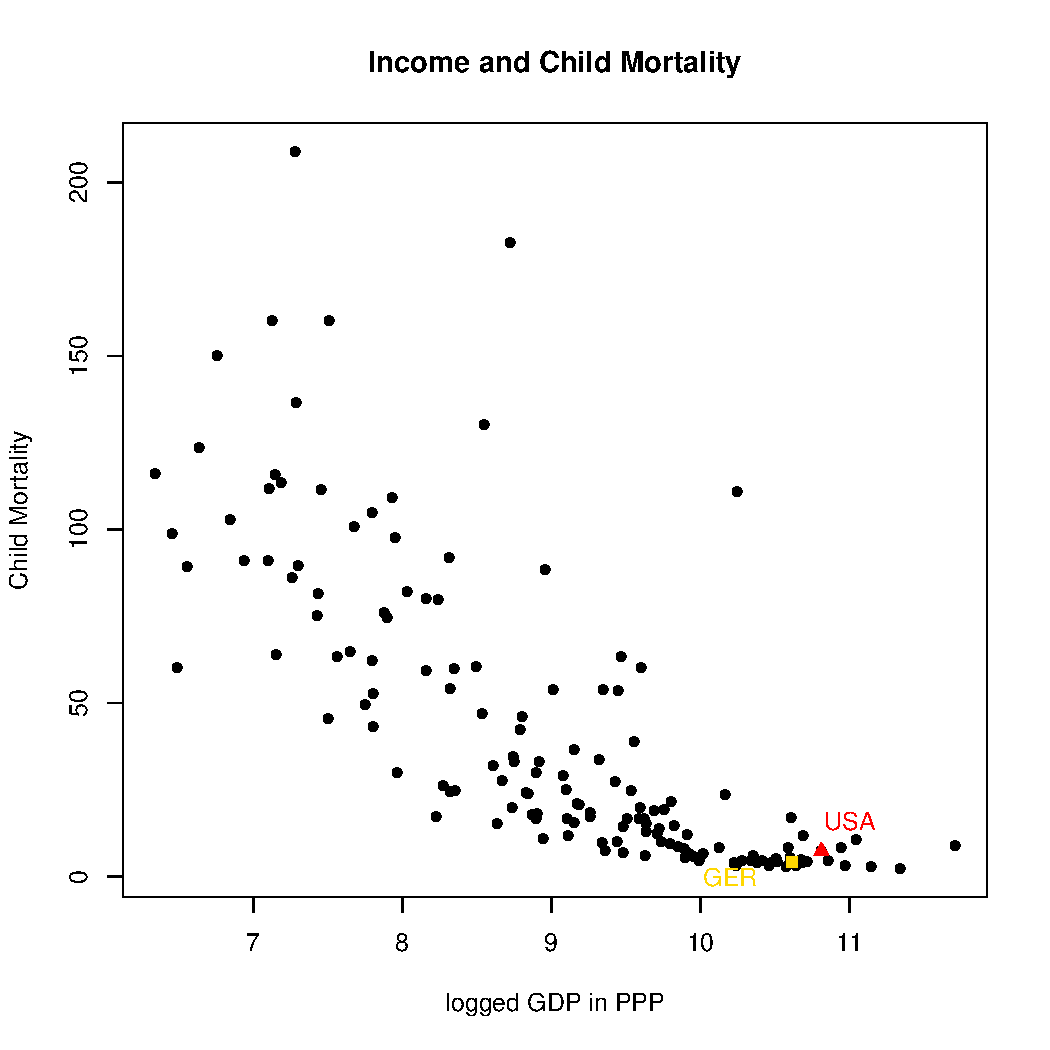
\includegraphics[width=8cm]{/Users/florianhollenbach/Documents/GitHub/Polisci209_2018/slides/week5/scatter_points.pdf}
\end{center}
\end{frame}


\begin{frame}[label={sec:orgce78a43}]{Bivariate Relationships in Numbers}
\begin{itemize}
\item How can we quantify the relationship between two continuous variables?
\end{itemize}

\pause
\begin{itemize}
\item Correlation: the most used measure of bivariate relationships
\item Correlation measures how two variables move together relative to their respective means.
\end{itemize}
\end{frame}

\begin{frame}[label={sec:org741a462}]{Calculating correlations -- Step 1: Standardizing a variable}
\begin{itemize}
\item By standardizing we bring all variables on the same scale
\item The resulting mean will be zero, the standard deviation will be one
\item We standardize by subtracting a variables mean and dividing by the standard deviation
\end{itemize}
\end{frame}

\begin{frame}[label={sec:org3bfe001}]{Calculating correlations -- Step 1: Standardizing a variable}
\begin{itemize}
\item Standardized variables are also called z-scores:
\end{itemize}
\(z_{i} = \frac{x_{i} - \bar{x} \text{(mean of x)}}{sd_{x} \text{(standard deviation of x)}}\)

\begin{itemize}
\item The z-score is independent of the scale of the variable or shifts in the variable
\end{itemize}
\pause

\begin{itemize}
\item This means GDP and (GDP*100 + 10000) will have the exact same z-scores
\end{itemize}
\end{frame}

\begin{frame}[label={sec:org6e9f410}]{Calculating correlations -- Step 2: Calculating the correlation}
Correlation (x,y) \(= \frac{1}{N} \sum^{N}_{i=1}\) z-score of \(x_i \times\) z-score of \(y_{i}\)

\pause

Correlation (x,y) \(= \frac{1}{N} \sum^{N}_{i=1} \frac{x_{i} - \bar{x}}{sd_{x}} \times   \frac{y_{i} - \bar{y}}{sd_{y}}\)
\end{frame}

\begin{frame}[label={sec:org3d4f517}]{Calculating correlations -- Step 3: Interpretation}
\begin{itemize}
\item Correlation measures \emph{linear} association
\item Correlations are between \(-1\) and \(1\)
\end{itemize}
\end{frame}

\begin{frame}[fragile,label={sec:org35ffccc}]{Calculating correlations -- Step 3: Interpretation}
 \begin{verbatim}
cor(log(data$GDP),data$Child.Mortality, use = "pairwise")
\end{verbatim}

= -0.7684907
\end{frame}

\begin{frame}[label={sec:org10e3a63}]{Calculating correlations -- Step 3: Interpretation}
cor(data[, c(``GDP'', ``Child.Mortality'', ``PolityIV'')], use = ``pairwise.complete.obs'')
\end{frame}

\begin{frame}[fragile,shrink=45,label={sec:org3594557}]{Calculating correlations -- Step 3: Interpretation}
 \begin{verbatim}
### by hand
z_gdp <- (log(data$GDP) - mean(log(data$GDP), na.rm = T))/sd(log(data$GDP), na.rm =T)
z_CM <- (data$Child.Mortality - mean(data$Child.Mortality, na.rm = T))/sd(data$Child.Mortality, na.rm =T)
cor <- sum(z_gdp*z_CM)/(length(z_gdp)-1)
 -0.7684907
\end{verbatim}
\end{frame}
\end{document}